\documentclass{amsart}
\usepackage{amsmath}
\usepackage{amsfonts}
\usepackage{amssymb}
\usepackage{amsthm}
\usepackage{graphicx}
\usepackage{tikz}
\usepackage{tkz-euclide}
\usetikzlibrary{intersections}
\usetikzlibrary{
  knots,
  hobby,
  decorations.pathreplacing,
  shapes.geometric,
  calc,
  positioning
}
%\usetikzlibrary{arrows,chains,matrix,positioning,scopes,knots,shapes,spy,snakes}


\theoremstyle{plain}
\newtheorem{theorem}{Theorem}[section]
\newtheorem{lemma}[theorem]{Lemma}
\newtheorem{proposition}[theorem]{Proposition}
\newtheorem{corollary}{Corollary}[section]

\theoremstyle{definition}
\newtheorem{definition}{Definition}[section]
\newtheorem{conjecture}{Conjecture}[section]
\newtheorem{example}{Example}[section]
\newtheorem{claim}{Claim}[section]

\theoremstyle{remark}
\newtheorem{exercise}{Exercise}
\newtheorem*{note}{Note}

\begin{document}

\title{Complex Analysis}
\author{Danny B}
\date{February 20, 2016}


\section{Basic Concepts in Topology}

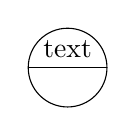
\begin{tikzpicture}
  \draw circle (0.5);
  \draw (-0.5, 0) to ["text"] (0.5, 0);
\end{tikzpicture}

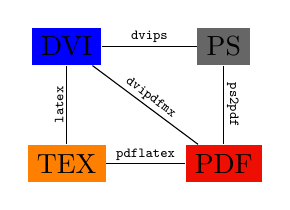
\begin{tikzpicture}
  [every edge quotes/.style = {text=black, auto, font = \tiny\ttfamily, inner sep=1pt, sloped}]
  \node (tex) [fill=orange] {TEX};
  \node (pdf) [fill={rgb:red,244;green,15;blue,2}, right=of tex] {PDF};
  \node (dvi) [fill=blue, above=of tex] {DVI};
  \node (ps)  [fill=black!60, above=of pdf] {PS};
  \draw (tex) edge["pdflatex"] (pdf)
    (tex) edge["latex"] (dvi)
    (dvi) edge["dvips"] (ps)
    (dvi) edge["dvipdfmx"] (pdf)
    (ps) edge["ps2pdf"] (pdf);
\end{tikzpicture}

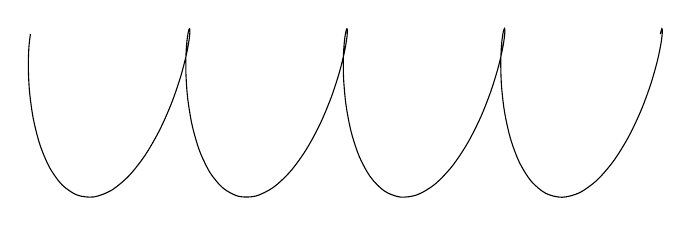
\begin{tikzpicture}
  \draw [domain=-4*pi:4*pi, samples=80, smooth]
    plot (\x/pi, {cos(\x r)}, {sin(\x r)}) ;
\end{tikzpicture}

\begin{tikzpicture}
  \foreach \k in {0,2}
    {\draw plot (\x + \k, \x^2);}
\end{tikzpicture}

\begin{definition}
A Topological Space blah $(\mathcal{X}, \mathcal{T})$ is a set $\mathcal{X}$ with a family $\mathcal{T}$ of subsets of $\mathcal{T}$ such that:
\begin{enumerate}
 \item $\mathcal{X} \in \mathcal{T}$
\end{enumerate}
\end{definition}


\end{document}
